\begin{frame}
{\textbf{Problem:3}\\In $\Delta$ABC, D and E are two points on BC such that BD = DE = EC. Show that ar(ABD) = ar(ADE) = ar(AEC).}
\begin{itemize}
\item \textbf{Solution:}
\end{itemize}
\textbf{Given:}\\
$\Delta$ABC where DE = DB = EC\\
Prove ar(ABD) = ar(ADE) = ar(AEC) \& take AL = Altitude of $\Delta$ABC\\
 Area of $\Delta$ ABC \begin{align}= \frac{1}{2}\times BD \times AL  \end{align}
 Area of $\Delta$ ADE \begin{align} = \frac{1}{2}\times DE \times AL \end{align}
\end{frame}
\begin{frame}
Area of $\Delta$ AEC \begin{align}= \frac{1}{2}\times EC \times AL \end{align}
By solving Equations (11), (12) we get,\\
$\frac{1}{2}\times$ BD $\times$ AL = $\frac{1}{2}\times$ DE $\times$ AL,\\ 
BD = DE. \\\enspace
By solving Equations (12), (13) we get,\\
$\frac{1}{2}\times$ BD $\times$ AL = $\frac{1}{2}\times$ EC $\times$ AL,\\
BD = EC. \\
from solving equations (11),(12) and (13) \\
BD = DE = EC\\\enspace
then, ar(ABD) = ar(ADE) = ar(AEC).\\\enspace
the python code for  Figure 0-5 is codes/tri\_area.py\\
and the equivalent latex-tikz code for Figure 0-6 is tri\_area.tex
\end{frame}
\begin{frame}{}
\begin{figure}[!ht]
	\begin{center}
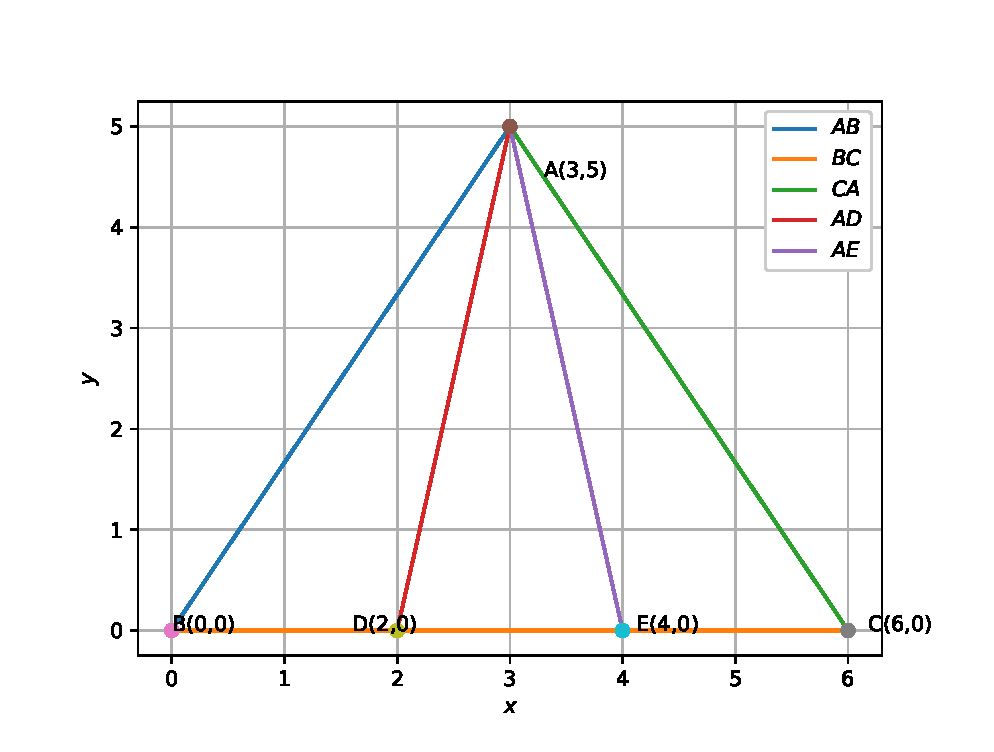
\includegraphics[width=0.8\columnwidth]{./figs/tri_area.eps}
	\end{center}
	\caption{}
	\label{}	
\end{figure}
\end{frame}
\begin{frame}{}
\begin{figure}[!ht]
	\begin{center}
		\resizebox{0.8\columnwidth}{!}{\begin{tikzpicture}[scale=1]

%Triangle sides
\def\a{6}
\def\b{4}
\def\c{2}
\def\d{3}
\def\e{5}
%Marking coordiantes
\color{blue}
\coordinate [label=above:$A$] (A) at (\d,\e);
\coordinate [label=below:$B$] (B) at (0,0);
\coordinate [label=below:$C$] (C) at (\a,0);
\coordinate [label=below:$D$] (D) at (\c,0);
\coordinate [label=below:$E$] (E) at (\b,0);

%Drawing triangle ABC
\color{black}
\draw (A) -- node[right] {$\textrm{}$} (B) -- node[below] {$\textrm{}$} (C) -- node[right,,xshift=2mm] {$\textrm{}$} (A)-- node[below] {$\textrm{}$} (E) (A)-- node[below] {$\textrm{}$} (D) ;
\end{tikzpicture}
}
	\end{center}
	\caption{}
	\label{}	
\end{figure}
\end{frame}
\begin{frame}
\textbf{Coordinates of  Triangle:}
\begin{enumerate}
\item Construct triangle ABC and ADB and AEC with a = 5, b = 6, c = 3.
\item where D = $\frac{B+E}{2}$ and E = $\frac{D+C}{2}$.
\item The vertices of $\Delta$ABC are A = $\begin{pmatrix} c\\a \end{pmatrix}$, B = $\begin{pmatrix} 0\\0 \end{pmatrix}$, C = $\begin{pmatrix} b\\0 \end{pmatrix}.$ 
\end{enumerate}
\url{https://github.com/Narendrapulipati/geometry/blob/master/codes/tri_area.py}
\url{https://github.com/Narendrapulipati/geometry/blob/master/figs/tri_area.tex}
\end{frame}